\documentclass[10pt,aspectratio=43]{beamer}
\beamertemplatenavigationsymbolsempty
\setbeamertemplate{footline}[page number]
\usefonttheme[onlymath]{serif}
\setbeamersize{text margin left=0.6cm, text margin right=0.6cm}
\setbeamerfont{frametitle}{size=\Large}
\setbeamertemplate{itemize items}[triangle]
\setbeamertemplate{enumerate items}[default]

\usepackage[utf8]{inputenc}
\usepackage[english,russian]{babel}
\usepackage{amssymb,amsfonts,amsmath,mathtext}
\usepackage{subfig}
\usepackage{array}
\usepackage{bm}
\usepackage{multicol}
\usepackage{hyperref}
\usepackage{hhline}
\usepackage{subcaption}
\usepackage{accents}
\usepackage{booktabs}
\usepackage{colortbl}
\usepackage{mathtools}
\usepackage{graphicx}
\usepackage{adjustbox}
\usepackage{ragged2e}
\usepackage{tikz}
\usetikzlibrary{positioning,arrows.meta,calc,overlay-beamer-styles}

% latin bold lower
\newcommand{\ba}{\mathbf{a}} 
\newcommand{\bc}{\mathbf{c}} 
\newcommand{\be}{\mathbf{e}} 
\newcommand{\bh}{\mathbf{h}} 
\newcommand{\bp}{\mathbf{p}} 
\newcommand{\bt}{\mathbf{t}} 
\newcommand{\bs}{\mathbf{s}} 
\newcommand{\bu}{\mathbf{u}} 
\newcommand{\bv}{\mathbf{v}} 
\newcommand{\bw}{\mathbf{w}} 
\newcommand{\bx}{\mathbf{x}} 
\newcommand{\by}{\mathbf{y}} 
\newcommand{\bz}{\mathbf{z}} 

% latin bold upper
\newcommand{\bA}{\mathbf{A}} 
\newcommand{\bB}{\mathbf{B}} 
\newcommand{\bC}{\mathbf{C}} 
\newcommand{\bI}{\mathbf{I}} 
\newcommand{\bJ}{\mathbf{J}} 
\newcommand{\bL}{\mathbf{L}} 
\newcommand{\bM}{\mathbf{M}} 
\newcommand{\bP}{\mathbf{P}}
\newcommand{\bQ}{\mathbf{Q}} 
\newcommand{\bR}{\mathbf{R}} 
\newcommand{\bT}{\mathbf{T}} 
\newcommand{\bU}{\mathbf{U}} 
\newcommand{\bV}{\mathbf{V}} 
\newcommand{\bW}{\mathbf{W}} 
\newcommand{\bX}{\mathbf{X}} 
\newcommand{\bY}{\mathbf{Y}} 
\newcommand{\bZ}{\mathbf{Z}} 

% latin cal upper
\newcommand{\cF}{\mathcal{F}} 
\newcommand{\cG}{\mathcal{G}} 
\newcommand{\cI}{\mathcal{I}} 
\newcommand{\cL}{\mathcal{L}} 
\newcommand{\cM}{\mathcal{M}} 
\newcommand{\cN}{\mathcal{N}} 
\newcommand{\cS}{\mathcal{S}} 
\newcommand{\cT}{\mathcal{T}} 
\newcommand{\cW}{\mathcal{W}} 
\newcommand{\cX}{\mathcal{X}} 
\newcommand{\cZ}{\mathcal{Z}} 

% latin bb upper
\newcommand{\bbE}{\mathbb{E}} 
\newcommand{\bbI}{\mathbb{I}} 
\newcommand{\bbP}{\mathbb{P}} 
\newcommand{\bbR}{\mathbb{R}}
\newcommand{\bbX}{\mathbb{X}} 
\newcommand{\bbY}{\mathbb{Y}}
\newcommand{\bbW}{\mathbb{W}} 

% greek bold lower
\newcommand{\bepsilon}{\boldsymbol{\epsilon}} 
\newcommand{\btheta}{\boldsymbol{\theta}} 
\newcommand{\blambda}{\boldsymbol{\lambda}} 
\newcommand{\bpi}{\boldsymbol{\pi}} 
\newcommand{\bmu}{\boldsymbol{\mu}} 
\newcommand{\bsigma}{\boldsymbol{\sigma}} 
\newcommand{\bphi}{\boldsymbol{\phi}} 

% greek bold upper
\newcommand{\bSigma}{\boldsymbol{\Sigma}} 

\DeclareMathOperator*{\argmin}{arg\,min}
\DeclareMathOperator*{\argmax}{arg\,max}

% transpose
\newcommand{\T}{^{\text{\tiny\sffamily\upshape\mdseries T}}}


\newcommand{\bb}{\mathbf{b}}
\newcommand{\bq}{\mathbf{q}}
\newcommand{\bS}{\mathbf{S}}
\newcommand{\bH}{\mathbf{H}}

\newcommand{\bE}{\mathbf{E}}
\newcommand{\bF}{\mathbf{F}}
\newcommand{\bomega}{\boldsymbol{\omega}}

\newcommand{\bgamma}{\boldsymbol{\gamma}}
\newcommand{\bdelta}{\boldsymbol{\delta}}
\newcommand{\bPsi}{\boldsymbol{\Psi}}
\newcommand{\bpsi}{\boldsymbol{\psi}}
\newcommand{\bxi}{\boldsymbol{\xi}}
\newcommand{\bchi}{\boldsymbol{\chi}}
\newcommand{\bzeta}{\boldsymbol{\zeta}}
\newcommand{\beps}{\boldsymbol{\varepsilon}}
\newcommand{\bZeta}{\boldsymbol{Z}}
% mathcal

\newcommand{\cY}{\mathcal{Y}}
\newcommand{\dH}{\mathds{H}}
\newcommand{\dR}{\mathds{R}}
\DeclareMathOperator{\spn}{span}

% Цвет структуры стандартной темы beamer (синий заголовков).
\definecolor{sblue}{rgb}{0.2,0.2,0.7}
% Заголовок внутри слайда: цвет темы, без плашки и тени (как у Тихонова).
\newcommand{\shead}[1]{\vspace{3pt}{\color{sblue}\large #1}\par\vspace{2pt}}
% Вывод слайда: обычный текст, прижатый к нижнему краю.
\newcommand{\takeaway}[1]{\par\vfill{\justifying #1\par}}

% Цвета отображений как на рисунке касательного пространства.
\definecolor{logc}{RGB}{0,0,220}
\definecolor{expc}{RGB}{210,0,0}
\definecolor{geoc}{RGB}{0,140,0}
% Цвета трех осей работы: время, пространство, модальности.
\definecolor{ctime}{RGB}{204,102,0}
\definecolor{cspace}{RGB}{0,125,95}
\definecolor{cmod}{RGB}{125,40,160}
% Акцентный цвет для ключевой части формулы; используется редко.
\definecolor{accent}{RGB}{204,102,0}
\newcommand{\hl}[1]{{\color{accent}#1}}
\usepackage[hyperlink]{qrcode}
% Светлая заливка лучшей строки таблицы тем же акцентом.
\newcommand{\bestrow}{\rowcolor{accent!12}}

\title[Пространственно-временные методы декодирования]{Пространственно-временные методы декодирования
мультимодальных многомерных временных рядов}
\author[Д.\,Д.~Дорин]{Даниил Дмитриевич Дорин}
\institute{Диссертация на соискание ученой степени\\
кандидата физико-математических наук\\[2pt]
1.2.1~--- Искусственный интеллект и машинное обучение\\[2pt]
Научный руководитель: к.ф.-м.н. А.\,В.~Грабовой}
\date{Москва~--- 2026}

\begin{document}

\begin{frame}
\thispagestyle{empty}
\maketitle
\end{frame}
%----------------------------------------------------------------------------------------------------------
\begin{frame}[t]{\large Пространственно-временные методы декодирования мультимодальных многомерных временных рядов}
\justifying
Исследуется задача декодирования: сигнал задан измерениями, реакция порождена внешним воздействием, требуется восстановить воздействие по измерениям. Выборка \textcolor{sblue}{ограничена}, а отклик \textcolor{cspace}{избыточен по пространству} и \textcolor{ctime}{запаздывает во времени} относительно воздействия.

\shead{Задача}
Построить отображение декодирования, опирающееся на \textcolor{ctime}{временную}, \textcolor{cspace}{пространственную} и \textcolor{cmod}{межмодальную} структуру.

\shead{Метод решения}
\begin{enumerate}
\justifying
    \item \textcolor{ctime}{Время:} лаг отклика оценивается по ошибке прогноза сигнала.
    \item \textcolor{cspace}{Пространство:} отбор информативных каналов, ковариация как точка риманова многообразия.
    \item \textcolor{cmod}{Модальности:} вторая дополняет первую и повышает качество.
\end{enumerate}
\takeaway{Методы формулируются для любых многоканальных рядов и проверяются на функциональной магнитно-резонансной томографии (фМРТ) и электроэнцефалографии (ЭЭГ) при визуальной стимуляции.}
\end{frame}
%----------------------------------------------------------------------------------------------------------
\begin{frame}{Постановка задачи}
\justifying
Пусть $\mathcal{X}_{(m)}$ обозначает пространство наблюдений модальности $m$, где $m = 1, \ldots, M$.
Тогда совместное пространство данных
\[
\mathcal{X} = \mathcal{X}_{(1)} \times \ldots \times \mathcal{X}_{(M)}.
\]
Внешний стимул или его характеристика $\mathbf{y} \in \mathcal{Y}$.
Требуется построить отображение декодирования
\[
\mathbf{g}: \mathcal{X} \rightarrow \mathcal{Y}.
\]

\shead{Решаемые задачи}
Классификация временных рядов фМРТ по категориям стимулов
\[
\mathbf{g}: \mathcal{X}_{f} \rightarrow \{1,\ldots,C\}.
\]
Реконструкция изображений по совместным сигналам фМРТ--ЭЭГ
\[
\mathbf{g}: \mathcal{X}_{f} \times \mathcal{X}_{e} \rightarrow \mathcal{Y}.
\]
\end{frame}
%----------------------------------------------------------------------------------------------------------
\begin{frame}[t]{Оценка гемодинамического лага}
\justifying
Скан фМРТ $\mathbf{F}(t)$ соответствует кадру $\mathbf{y}(t - \Delta t)$, предъявленному на гемодинамический лаг $\Delta t$ раньше. Лаг оценивается по качеству прогноза фМРТ-отклика по стимулу в обратной к декодированию задаче.

\shead{Линейная авторегрессионная модель}
Приращение скана $\boldsymbol{\delta}(t) = \mathbf{F}(t) - \mathbf{F}(t-1)$ линейно по эмбеддингу $\mathbf{x}(t)$ кадра $\mathbf{y}(t - \Delta t)$, полученному предобученным энкодером:
\[
\widehat{\boldsymbol{\delta}}(t) = \widehat{\mathbf{W}}\,\mathbf{x}(t), \qquad
\widehat{\mathbf{W}}(\Delta t) = \argmin_{\mathbf{W}} \sum_{t} \big\| \boldsymbol{\delta}(t) - \mathbf{W}\mathbf{x}(t) \big\|_2^2 + \lambda \|\mathbf{W}\|_F^2 .
\]
Лаг выбирается по минимуму MSE на тестовой выборке.
\begin{center}
    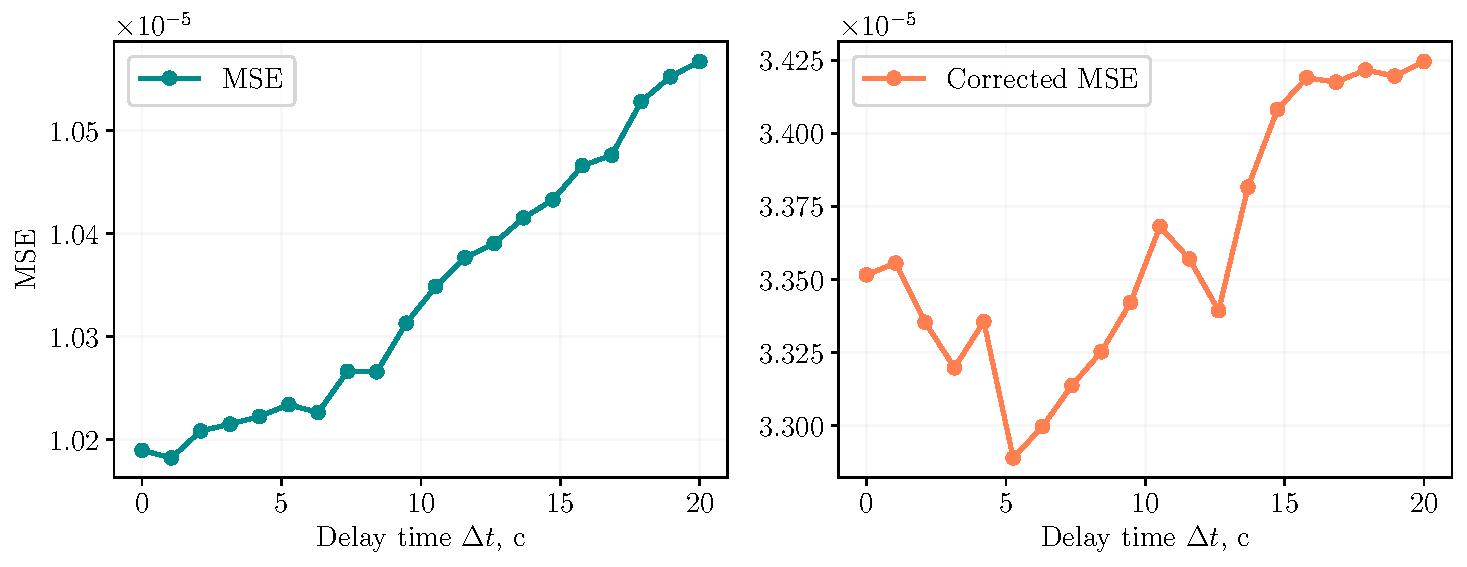
\includegraphics[width=0.64\linewidth]{figs/Figure_1.pdf}
\end{center}
\takeaway{На зрительной коре минимум MSE выражен отчетливо, а найденный лаг согласуется с физиологией BOLD-отклика.}
\end{frame}
%----------------------------------------------------------------------------------------------------------
\begin{frame}[t]{Метод классификации: признаки соответствия классам}
\justifying
Заданы ряды фМРТ $\mathbf{S}_i$ одного испытуемого с метками $y_i \in \{1, \ldots, L\}$; ищется классификатор $\mathbf{h}: \mathcal{X}_s \to \{1, \ldots, L\}$. Маски классов строит алгоритм кросс-корреляции сигнала со стимулом при лаге $\Delta t$.
\begin{center}
    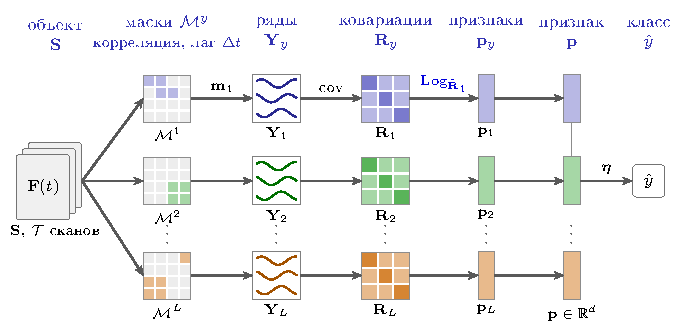
\includegraphics[width=0.9\linewidth]{figs/Figure_2.pdf}
\end{center}
\takeaway{Ковариация $\mathbf{R}_y$ рядов области проецируется отображением $\operatorname{Log}$ в точке среднего $\bar{\mathbf{R}}_y$ класса; вектор $\mathbf{p}_y$ измеряет соответствие объекта классу $y$, признаки всех классов конкатенируются.}
\end{frame}
%----------------------------------------------------------------------------------------------------------
\begin{frame}[t]{Проекция на риманово касательное пространство}
\justifying
Ковариация $\mathbf{R}_j$ проецируется на касательное пространство $T_{\mathbf{R}}$ в точке $\mathbf{R}$ отображением $\textcolor{logc}{\operatorname{Log}_{\mathbf{R}}}$ и возвращается на многообразие $\mathcal{R}$ отображением $\textcolor{expc}{\operatorname{Exp}_{\mathbf{R}}}$; длина геодезической между $\mathbf{R}$ и $\mathbf{R}_j$ равна $\textcolor{geoc}{\delta_{\mathcal{R}}(\mathbf{R}, \mathbf{R}_j)}$.
\begin{center}
    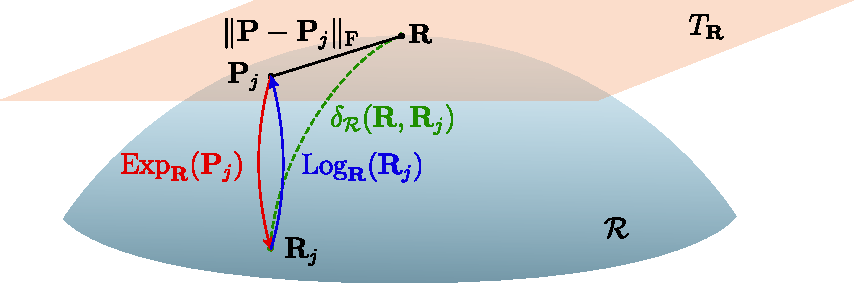
\includegraphics[width=0.7\linewidth]{figs/Figure_3.pdf}
\end{center}
\vspace{-0.4em}
\begin{align*}
\textcolor{logc}{\operatorname{Log}_{\mathbf{R}}(\mathbf{R}_j)} &= \mathbf{R}^{\frac{1}{2}} \log\big(\mathbf{R}^{-\frac{1}{2}}\mathbf{R}_j\mathbf{R}^{-\frac{1}{2}}\big) \mathbf{R}^{\frac{1}{2}} \in T_{\mathbf{R}}, \\[-1pt]
\textcolor{expc}{\operatorname{Exp}_{\mathbf{R}}(\mathbf{P}_j)} &= \mathbf{R}^{\frac{1}{2}} \exp\big(\mathbf{R}^{-\frac{1}{2}}\mathbf{P}_j\mathbf{R}^{-\frac{1}{2}}\big) \mathbf{R}^{\frac{1}{2}} \in \mathcal{R}, \\[-1pt]
\textcolor{geoc}{\delta_{\mathcal{R}}(\mathbf{R}, \mathbf{R}_j)} &= \big\| \log\big(\mathbf{R}^{-\frac{1}{2}}\mathbf{R}_j\mathbf{R}^{-\frac{1}{2}}\big) \big\|_F .
\end{align*}
Точкой касания служит риманово среднее ковариаций выборки $\mathbf{R} = \bar{\mathbf{R}}$.
\end{frame}
%----------------------------------------------------------------------------------------------------------
\begin{frame}{Сохранение расстояний и устойчивость проекции}
\begin{columns}[c]
\begin{column}{0.48\textwidth}
\justifying
\small
\shead{Теорема 1 (Дорин, 2026)}
Пусть $\delta_{\mathcal{R}}(\bar{\mathbf{R}}, \mathbf{R}_i) \leqslant \rho$ для всех $i$. Тогда норма признака равна геодезическому расстоянию до среднего, $\|\mathbf{p}_i\|_2 = \delta_{\mathcal{R}}(\bar{\mathbf{R}}, \mathbf{R}_i)$, а расстояния между признаками искажаются не более чем в $c(\rho) = \sinh(\rho/\sqrt{2})\big/(\rho/\sqrt{2})$ раз, и эта константа неулучшаема:
\vspace{-0.3em}
\[
\|\mathbf{p}_i - \mathbf{p}_j\|_2
\leqslant \delta_{\mathcal{R}}(\mathbf{R}_i, \mathbf{R}_j)
\leqslant c(\rho)\,\|\mathbf{p}_i - \mathbf{p}_j\|_2 .
\]

\shead{Теорема 2 (Дорин, 2026)}
Пусть $\hat{\mathbf{R}}$ выборочная ковариация по $\mathcal{T}$ гауссовским сканам с ковариацией $\mathbf{R} \in \mathbb{S}_{+}^{h}$. Тогда распределение $\delta_{\mathcal{R}}(\hat{\mathbf{R}}, \mathbf{R})$ не зависит от $\mathbf{R}$, и при $\varepsilon = \sqrt{h/\mathcal{T}} + t < 1$ с вероятностью не меньше $1 - 2e^{-\mathcal{T}t^2/2}$
\vspace{-0.3em}
\[
\delta_{\mathcal{R}}(\hat{\mathbf{R}}, \mathbf{R}) \;\leqslant\; \frac{2\sqrt{h}\,\varepsilon}{1-\varepsilon}
\;=\; O\big(h/\sqrt{\mathcal{T}}\big).
\]
\end{column}
\begin{column}{0.52\textwidth}
    \centering
    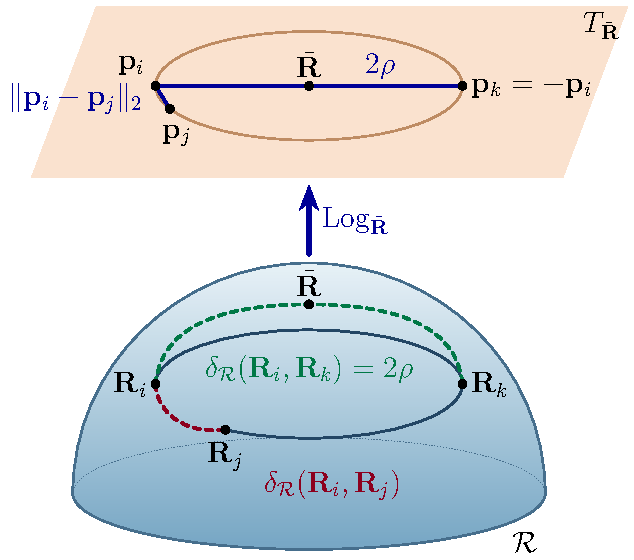
\includegraphics[width=\textwidth]{figs/Figure_4.pdf}
\end{column}
\end{columns}
\end{frame}
%----------------------------------------------------------------------------------------------------------
\begin{frame}[t]{Маски активности}
\justifying
\vspace{3mm}
Данные Haxby et al., первый испытуемый: частота сканирования $\mu = 2{,}5$~Гц, $h = 10$ областей, ядро $k_s = 4$.
\begin{figure}[h!]
	\centering
	\subfloat[\centering Алгоритм]{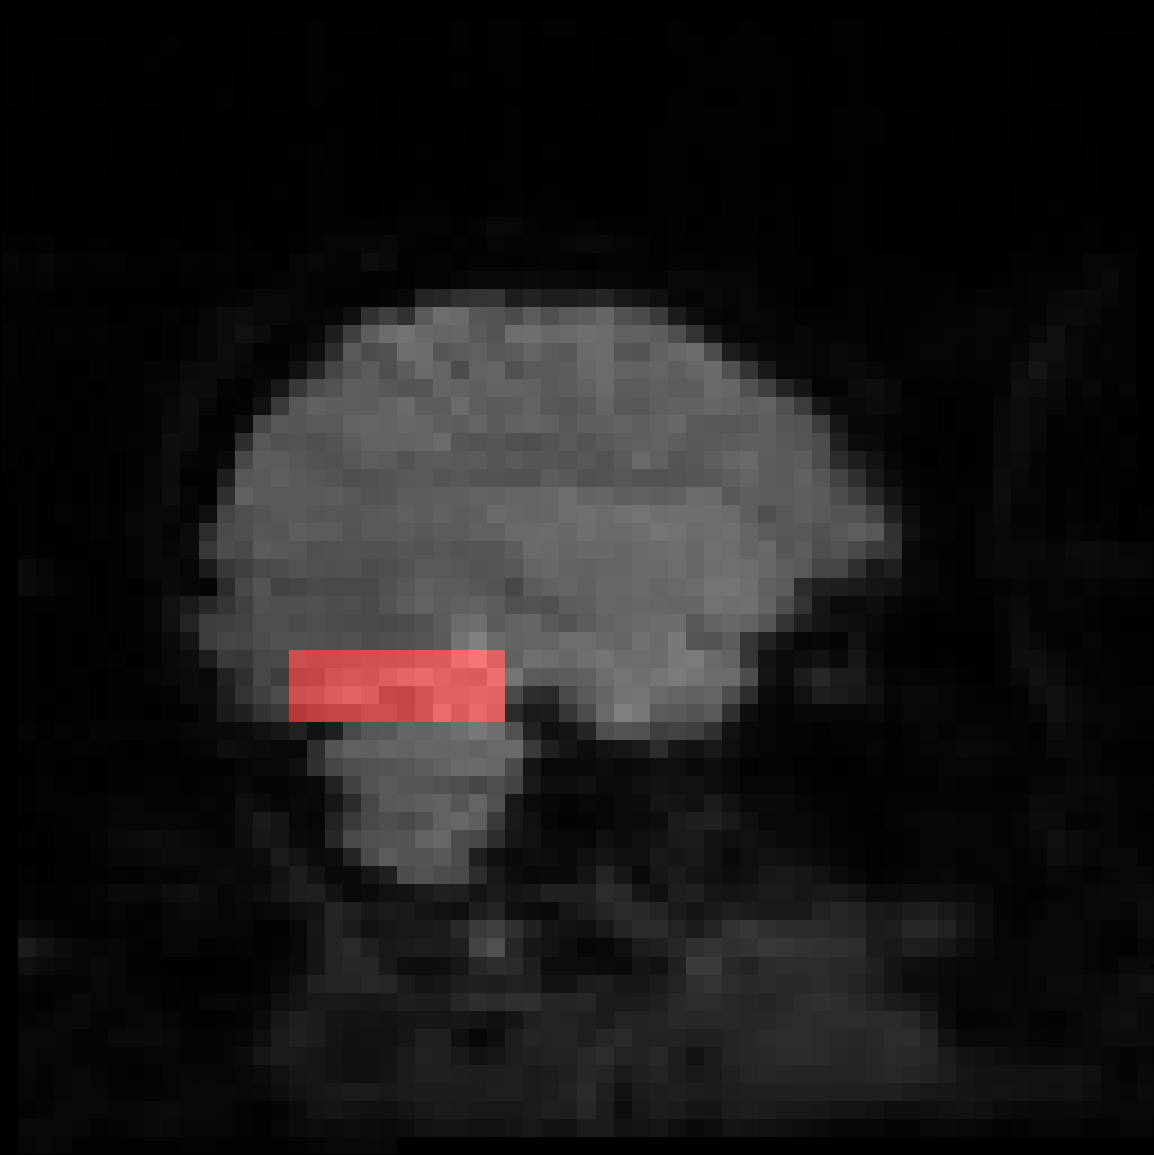
\includegraphics[width=0.3\textwidth]{figs/Figure_5.png}}\hfill
	\subfloat[\centering Статистически значимые области]{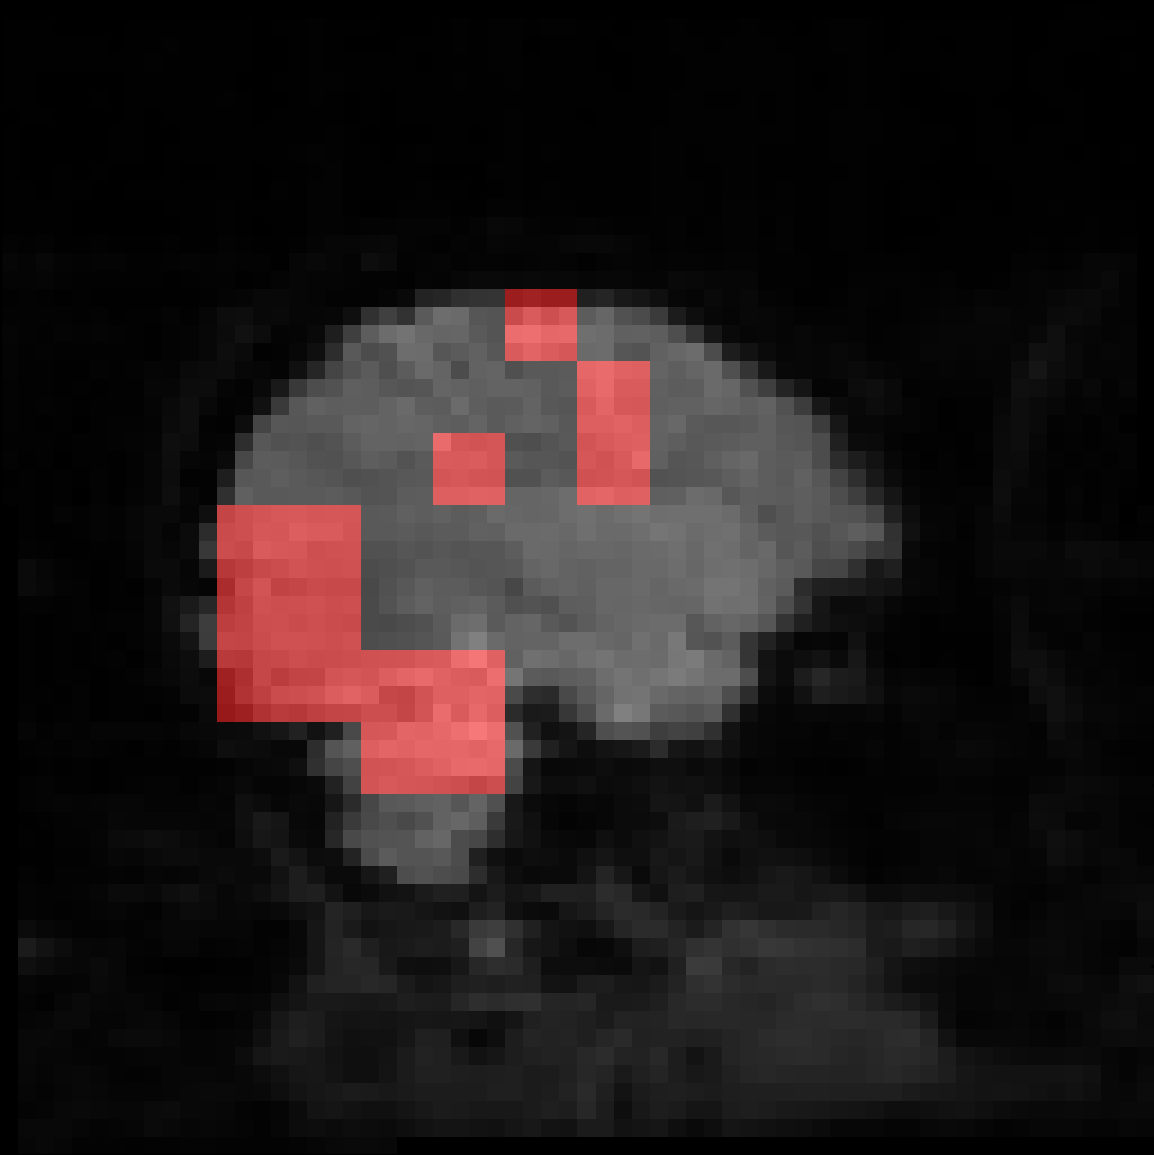
\includegraphics[width=0.3\textwidth]{figs/Figure_6.png}}\hfill
	\subfloat[\centering Разметка нейробиологов]{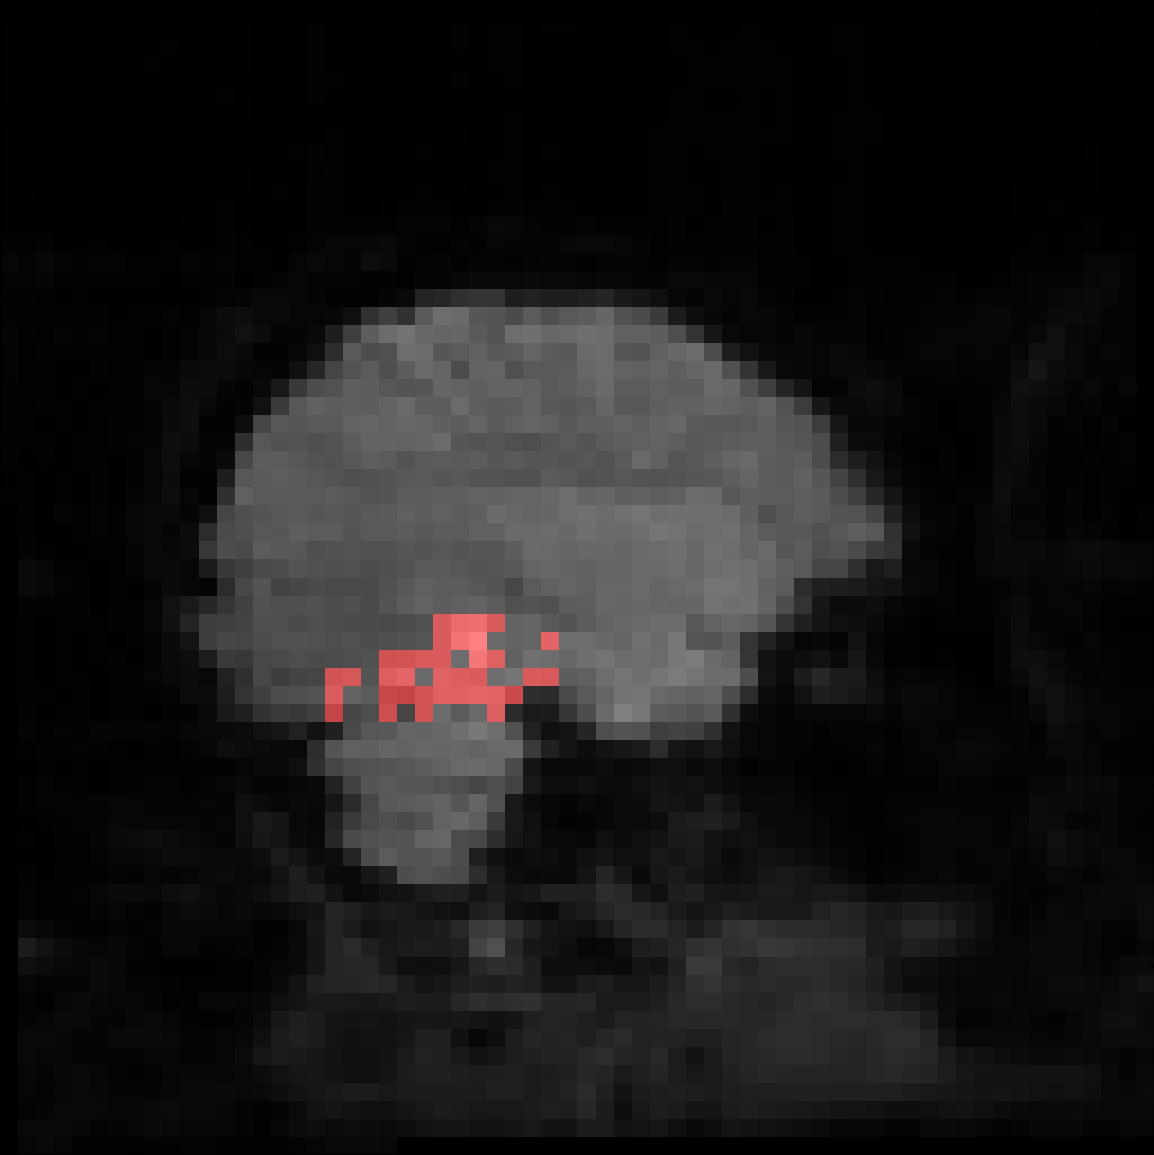
\includegraphics[width=0.3\textwidth]{figs/Figure_7.png}}
\end{figure}
\takeaway{Области, выделенные алгоритмом, покрывают разметку нейробиологов; корреляция отобранных вокселей со стимулом статистически значима.}
\end{frame}
%----------------------------------------------------------------------------------------------------------
\begin{frame}{Анализ компонент и сравнение с нейросетями}
\justifying
Рассматривается датасет Haxby et al., состоящий из данных 6 испытуемых, объем $N=96$, число классов $C=8$. Тест~--- 20\%. Метрики усреднены по 6 выборкам. Статистическая значимость обозначена *$p<.05$, **$p<.005$.

\medskip
\shead{Анализ исключением компонент} Три упрощенные модели, указаны $95\%$-е доверительные интервалы.
\par\nobreak\vspace{1.5mm}
\noindent\resizebox{\textwidth}{!}{%
\begin{tabular}{l ccc ccc}
    \toprule
    Method & Accuracy & Macro F1-Score & Micro F1-Score & Accuracy CI & Macro F1 CI & Micro F1 CI \\
    \midrule
    Ours, w/o TSM & 0.24 $\pm$ 0.11* & 0.22 $\pm$ 0.11* & 0.24 $\pm$ 0.11* & [0.11, 0.37] & [0.09, 0.36] & [0.10, 0.37] \\
    Ours, w/o Class Masks & 0.25 $\pm$ 0.13* & 0.23 $\pm$ 0.13* & 0.25 $\pm$ 0.13* & [0.09, 0.41] & [0.07, 0.39] & [0.09, 0.41] \\
    Ours, Original Mask & 0.10 $\pm$ 0.05** & 0.09 $\pm$ 0.04** & 0.10 $\pm$ 0.05** & [0.04, 0.16] & [0.03, 0.14] & [0.04, 0.16] \\
    \bestrow Ours & \textbf{0.61 $\pm$ 0.04} & \textbf{0.56 $\pm$ 0.03} & \textbf{0.61 $\pm$ 0.04} & [0.56, 0.66] & [0.52, 0.60] & [0.56, 0.66] \\
    \bottomrule
\end{tabular}}

\medskip
\shead{Сравнение с нейросетевыми решениями}
Нейросетевые модели LSTM и Attention на масках нейробиологов.
\par\nobreak\vspace{1.5mm}
\noindent\resizebox{\textwidth}{!}{%
\begin{tabular}{l ccc ccc}
    \toprule
    Model & Accuracy & Macro F1-Score & Micro F1-Score & Accuracy CI & Macro F1 CI & Micro F1 CI \\
    \midrule
    Original Mask \& LSTM & 0.12 $\pm$ 0.02** & 0.03 $\pm$ 0.01** & 0.12 $\pm$ 0.02** & [0.09, 0.14] & [0.02, 0.04] & [0.09, 0.14] \\
    Original Mask \& Attention & 0.14 $\pm$ 0.04** & 0.04 $\pm$ 0.03** & 0.14 $\pm$ 0.04** & [0.11, 0.18] & [0.02, 0.07] & [0.11, 0.18] \\
    \bestrow Ours, Logistic Regression $\bm{\varphi}$ & \textbf{0.61 $\pm$ 0.04} & \textbf{0.56 $\pm$ 0.03} & \textbf{0.61 $\pm$ 0.04} & [0.56, 0.66] & [0.52, 0.60] & [0.56, 0.66] \\
    \bottomrule
\end{tabular}}

\medskip
Исключение любой компоненты значимо снижает качество; на малой выборке метод превосходит нейросетевые модели.
\end{frame}
%----------------------------------------------------------------------------------------------------------
\begin{frame}{Мультимодальная реконструкция стимула}
\justifying
\vspace{2mm}
Задан датасет триплетов (фМРТ, ЭЭГ, изображение) $\mathfrak{D}=\{(\mathbf{F}_i,\mathbf{E}_i,\mathbf{I}_i)\}_{i=1}^{N}$; требуется построить отображение $\mathbf{f}: \mathcal{X}_f \times \mathcal{X}_e \to \mathcal{Y}$.
\begin{center}
    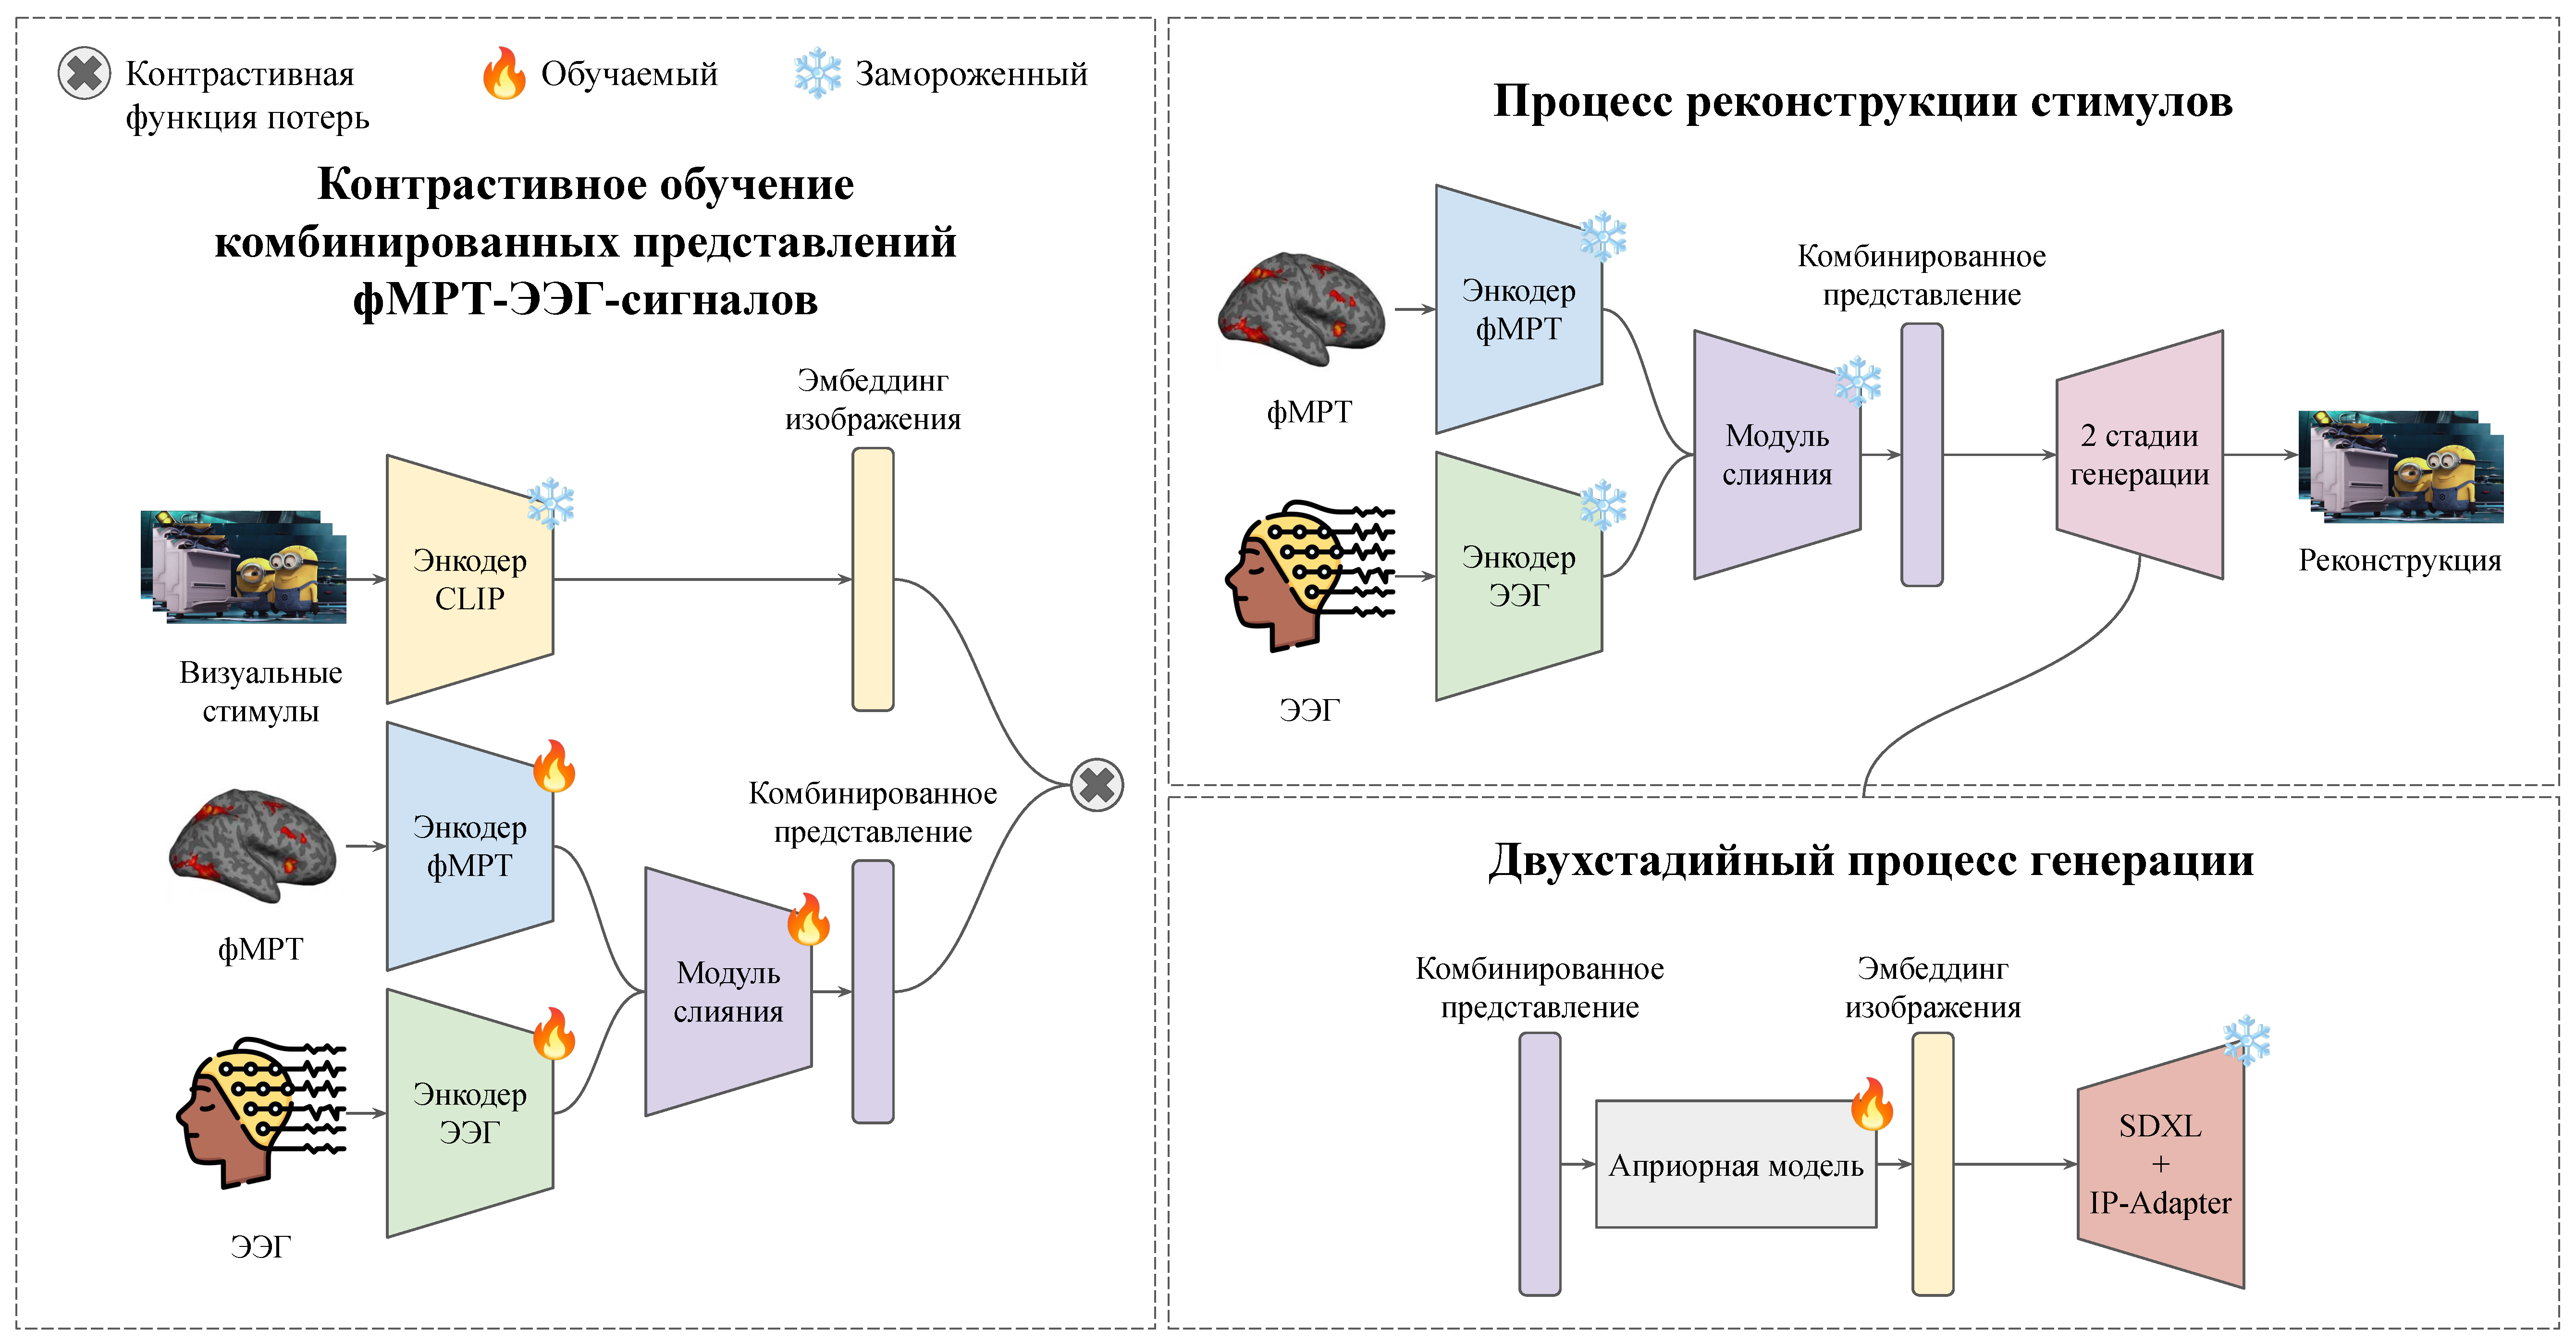
\includegraphics[width=0.93\linewidth]{figs/Figure_8.pdf}
\end{center}
\takeaway{Первый этап выравнивает объединенные представления фМРТ--ЭЭГ с эмбеддингами CLIP, второй порождает изображение двухстадийной диффузией, prior в пространстве CLIP и затем SDXL.}
\end{frame}
%----------------------------------------------------------------------------------------------------------
\begin{frame}[t]{Контрастивное выравнивание представлений}
\begin{columns}[c]
\begin{column}{0.56\textwidth}
\justifying
Батч из $B$ триплетов дает $B$ эмбеддингов изображений $\mathbf{Z}_I$ и $B$ объединенных эмбеддингов мозга $\mathbf{Z}_c$. После нормировки строк $\mathbf{Z}^n = \mathbf{Z} / \|\mathbf{Z}\|$ логиты равны косинусной близости с температурой $\tau$:
\[
\mathbf{L} = \mathbf{Z}_c^n \left(\mathbf{Z}_I^n\right)^{\T} e^{\tau}.
\]
Диагональ $\hl{\mathbf{L}_{bb}}$ отвечает верным парам, остальные $B^2 - B$ элементов служат отрицательными примерами без разметки.
\end{column}
\begin{column}{0.42\textwidth}
\centering
\begin{tikzpicture}[x=0.5cm, y=0.5cm, font=\scriptsize]
% cells: negatives light gray, row b blue, column b green, positives orange
\fill[black!7] (0,0) rectangle (5,-5);
\fill[logc!14] (0,-2) rectangle (5,-3);
\fill[geoc!16] (2,0) rectangle (3,-5);
\foreach \i in {0,...,4}{
    \fill[accent!85] (\i,-\i) rectangle ++(1,-1);
}
\foreach \i in {0,...,5}{
    \draw[white, line width=1pt] (\i,0) -- (\i,-5);
    \draw[white, line width=1pt] (0,-\i) -- (5,-\i);
}
\draw[black!40, line width=0.4pt] (0,0) rectangle (5,-5);
\node[text=white, font=\scriptsize] at (2.5,-2.5) {$\mathbf{L}_{bb}$};
% column indices (images) and row indices (brain signals)
\foreach \j/\t in {0/1, 1/2, 2/b, 3/{\cdots}, 4/B}{
    \node[anchor=south] at (\j+0.5,0.05) {$\t$};
}
\foreach \i/\t in {0/1, 1/2, 2/b, 3/{\vdots}, 4/B}{
    \node[anchor=east] at (-0.1,-\i-0.5) {$\t$};
}
\node[anchor=south, font=\footnotesize] at (2.5,0.55) {изображения $\mathbf{z}_I$ (CLIP)};
\node[anchor=south, rotate=90, font=\footnotesize] at (-0.65,-2.5) {сигналы мозга $\mathbf{z}_c$};
% legend
\node[anchor=north west, font=\scriptsize, align=left] at (-0.9,-5.35)
    {\tikz\fill[accent!85] (0,0) rectangle (0.25,0.25); положительные пары $\mathbf{L}_{bb}$\\[1pt]
     \tikz\fill[logc!40] (0,0) rectangle (0.25,0.25); строка $b$: выбор изображения\\[1pt]
     \tikz\fill[geoc!45] (0,0) rectangle (0.25,0.25); столбец $b$: выбор сигнала мозга};
\end{tikzpicture}
\end{column}
\end{columns}
\shead{Симметричная контрастивная функция потерь}
\vspace{-0.6em}
\[
\mathcal{L} = -\frac{1}{2B} \sum_{b=1}^{B} \left[
\log \frac{\exp(\hl{\mathbf{L}_{bb}})}{\textcolor{logc}{\sum_{j=1}^{B} \exp(\mathbf{L}_{bj})}}
+ \log \frac{\exp(\hl{\mathbf{L}_{bb}})}{\textcolor{geoc}{\sum_{i=1}^{B} \exp(\mathbf{L}_{ib})}}
\right]
\]
\medskip

Потери обучают энкодеры фМРТ и ЭЭГ и модуль объединения, сближая верные пары и раздвигая остальные в обоих направлениях.
\end{frame}
%----------------------------------------------------------------------------------------------------------
\begin{frame}{Оценка мультимодальной модели}
\justifying
Качество оценивается по CLIP-Score: косинусной близости объединенного эмбеддинга $\mathbf{z}_c$ и CLIP-эмбеддинга изображения $\mathbf{z}_I$,
\[
    \text{CLIP-Score}(\mathbf{z}_c, \mathbf{z}_I) = \frac{\langle \mathbf{z}_c, \mathbf{z}_I \rangle}{\| \mathbf{z}_c \| \| \mathbf{z}_I \|},
\]
усредненной по триплетам тестовой выборки для каждого испытуемого.

\begin{table}[h!]
    \centering
    
    \begin{tabular}{lccc}
        \toprule
        & \multicolumn{3}{c}{Название видеостимула} \\
        \cline{2-4}
        Модель & \texttt{monkey1} & \texttt{monkey2} & \texttt{monkey5} \\
        \midrule
        ЭЭГ & $0{,}231_{\pm 0{,}004}$ & $0{,}262_{\pm 0{,}004}$ & $0{,}224_{\pm 0{,}005}$ \\
        фМРТ & $0{,}254_{\pm 0{,}004}$ & $0{,}270_{\pm 0{,}003}$ & $0{,}242_{\pm 0{,}003}$ \\
        фМРТ--ЭЭГ & $0{,}310_{\pm 0{,}003}$ & $0{,}312_{\pm 0{,}004}$ & $0{,}284_{\pm 0{,}003}$ \\
        ЭЭГ \& Diffusion Prior & $0{,}542_{\pm 0{,}005}$ & $0{,}557_{\pm 0{,}003}$ & $0{,}538_{\pm 0{,}003}$ \\
        фМРТ \& Diffusion Prior & $0{,}564_{\pm 0{,}005}$ & $0{,}571_{\pm 0{,}004}$ & $0{,}551_{\pm 0{,}005}$ \\
        \bestrow фМРТ--ЭЭГ \& Diffusion Prior & $\textbf{0{,}668}_{\pm 0{,}003}$ & $\textbf{0{,}647}_{\pm 0{,}005}$ & $\textbf{0{,}644}_{\pm 0{,}003}$ \\
        \bottomrule
    \end{tabular}
\end{table}
Мультимодальная модель превосходит одномодальные аналоги.
\end{frame}
%----------------------------------------------------------------------------------------------------------
\begin{frame}{Примеры реконструкции}
\justifying
Реконструкция по одновременным записям фМРТ--ЭЭГ на тесте.
\begin{center}
    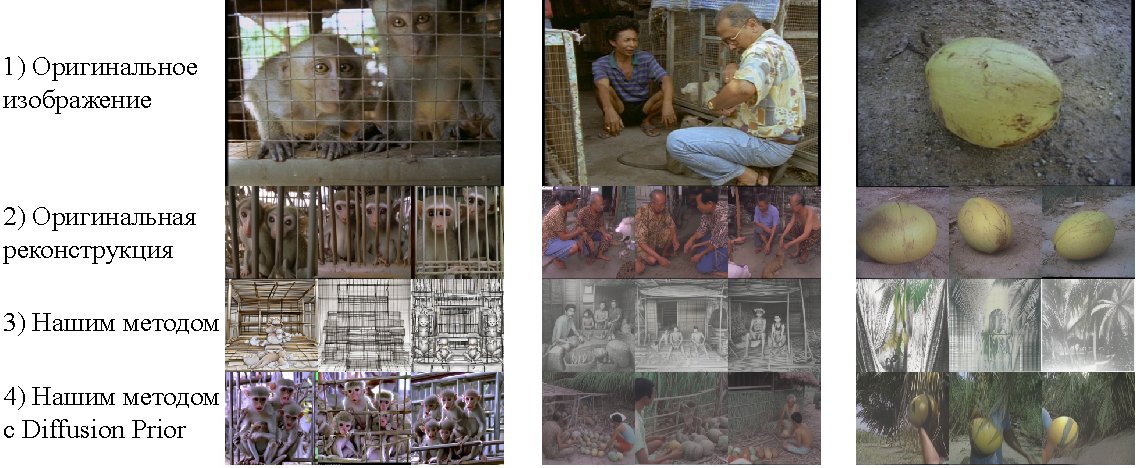
\includegraphics[width=0.9\linewidth]{figs/Figure_9.pdf}
\end{center}
Эмбеддинги CLIP обучены на парах изображение и текст, поэтому хранят семантику сцены и почти не хранят текстуры и пиксельные детали. Метод восстанавливает содержание стимула, а не его точный вид.
\end{frame}
%----------------------------------------------------------------------------------------------------------
\begin{frame}{Положения, выносимые на защиту}
\begin{enumerate}
\justifying
    \item Линейная авторегрессионная модель прогнозирования фМРТ-отклика по предъявленному стимулу и метод оценки гемодинамического лага BOLD-сигнала на ее основе.
    \item Метод классификации временных рядов фМРТ на основе масок активности классов и проекции ковариационных матриц на касательное пространство риманова многообразия, устойчивый в условиях ограниченного объема выборки одного пациента.
    \item Теоретические свойства проекции ковариационных матриц на касательное пространство в точке риманова среднего: инвариантность признаков к невырожденному преобразованию каналов, двусторонняя оценка искажения расстояний с неулучшаемой константой и оценка ошибки оценки ковариации по длине ряда.
    \item Мультимодальная архитектура реконструкции стимула по одновременным сигналам фМРТ и ЭЭГ с контрастивным выравниванием совместных представлений и двухстадийной диффузионной генерацией.
\end{enumerate}
\end{frame}
%----------------------------------------------------------------------------------------------------------
\begin{frame}{Публикации и апробация}
\shead{Публикации в журналах из перечня ВАК РФ, Scopus, WoS}
\begin{enumerate}
\footnotesize
\justifying
    \item \textit{\textbf{Dorin D.}, Kiselev N., Grabovoy A., Strijov V.} Forecasting fMRI Images From Video Sequences: Linear Model Analysis // Health Information Science and Systems.~--- 2024.
    \item \textit{\textbf{Dorin D.}, Grabovoy A., Strijov V.} Enhancing fMRI Data Decoding with Spatiotemporal Characteristics in Limited Dataset // Doklady Mathematics.~--- 2025.
    \item \textit{\textbf{Dorin D.}, Kiselev N., Grabovoy A.} Decoding Visual Information from Neural Signals: Image Reconstruction Based on Joint fMRI and EEG Analysis // Informatika i ee Primeneniya.~--- 2026.
\end{enumerate}
\shead{Доклады на международных и всероссийских конференциях}
\begin{enumerate}
\footnotesize
    \item 16-я Международная конференция <<Интеллектуализация обработки информации (ИОИ-2026)>>, Витебск, 28 сентября~--- 1 октября 2026.
    \item 68-я Всероссийская научная конференция МФТИ, Долгопрудный, 30 марта~--- 4 апреля 2026.
    \item X Международная конференция AI Journey 2025, Москва, 19--21 ноября 2025.
    \item 22-я Всероссийская конференция <<Математические методы распознавания образов (ММРО-2025)>>, Муром, 22--26 сентября 2025.
    \item 67-я Всероссийская научная конференция МФТИ, Долгопрудный, 31 марта~--- 5 апреля 2025.
    \item XXVI Международная конференция <<Нейроинформатика-2024>>, Долгопрудный, 21--25 октября 2024.
    \item 66-я Всероссийская научная конференция МФТИ, Долгопрудный, 1--6 апреля 2024.
\end{enumerate}
\end{frame}
%---------------------------------------------------------------------------------------------------------
\end{document}
